\documentclass[numberofslides]{AMSBeamer}
%% Options: 
%% numberofslides: show total number of slides
%% noAMSLogo: do not show AMS Logo


%\usepackage{import} %use includefrom instead import to use includeonly
%% include only specific texfile:
% \includeonly{subdirectory/texfile}
%% include only labeled frame:
% \includeonlyframes{title,label}


%% decrease title font if necessary
%\setbeamerfont{title}{series=\bfseries,size=\fontsize{14}{18}}

%% margins for title can also be changed:
% \makeatletter
% \setlength\title@titlemargin{13mm}\setlength\title@institutemargin\title@titlemargin
% \makeatother

%% Title:
\title[Navigation and Localization]{Navigation and Localization of the Hamster Robot}

%% Subtitle:
%\subtitle{Subtitle}

\author{Wiebke Outzen, Johnson Yarlagadda, Phillipp Grill and  Undine Holst}

\institute[Autonomous Multisensor Systems Group]{
	Autonomous Multisensor Systems Group \\
	Institute for Intelligent Cooperating Systems \\
	Faculty of Computer Science \\
	Otto von Guericke University Magdeburg
}
\mode<presentation>{\keywords{Schlüsselwörter durch Komma getrennt}}

\date{13.11.2023}%{Datum der Präsentation, \zB 1. Januar 2016}

\begin{document}


\begin{frame}[label=title]
	\maketitle
\end{frame}




%%%%%%%%%%%%%%%%%%%%%%%%%%%%%%%%%%%%%%%%%%%%%%%%%%%%%%%%%%%%%%%%%%%%%%%%%
%
% Slide without tikz or textblock
%
%%%%%%%%%%%%%%%%%%%%%%%%%%%%%%%%%%%%%%%%%%%%%%%%%%%%%%%%%%%%%%%%%%%%%%%%%


\begin{frame}[label=agenda]
  \frametitle{Agenda}
   \tableofcontents
\end{frame}

\section{Familiarization}
\begin{frame}[label=familiarization]
	\frametitle{\insertsectionhead}%
    \begin{itemize}
        \item ROS structure
        \item Controlling the robot via keyboard/joystick
        \item Teleop\_twist
    \end{itemize}
    \vspace{1cm}
    \begin{figure}
        \centering
        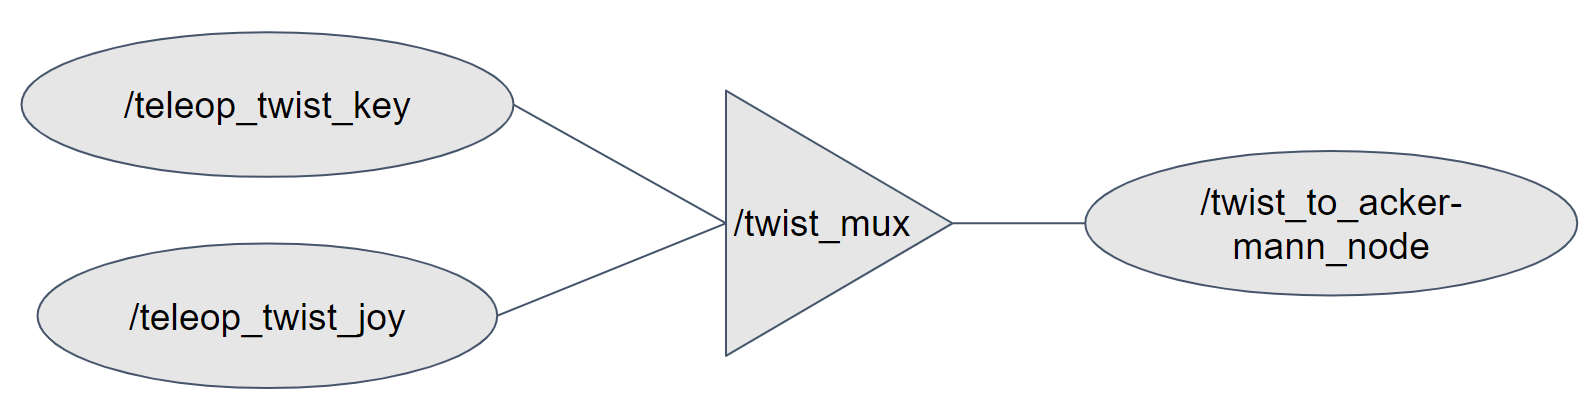
\includegraphics[width=12cm]{Presentations/LaTeX/images/Teleop_twist.png}
        \caption{Structure of the nodes}
    \end{figure}
\end{frame}

%---------------------------------------------------------------------

\subsection{Generate a map}
\begin{frame}[label=map]
	\frametitle{\insertsectionhead}%
    \begin{minipage}{0.5\textwidth}
        \textbf{\insertsubsectionhead}
        \begin{itemize}
            \item Slam\_gmapping
            \item Drive with controller until map in rviz is clear
            \item \texttt{map\_server} \texttt{map\_saver}
        \end{itemize}
    \end{minipage}%
    \begin{minipage}{0.5\textwidth}
        \begin{figure}
            \centering
                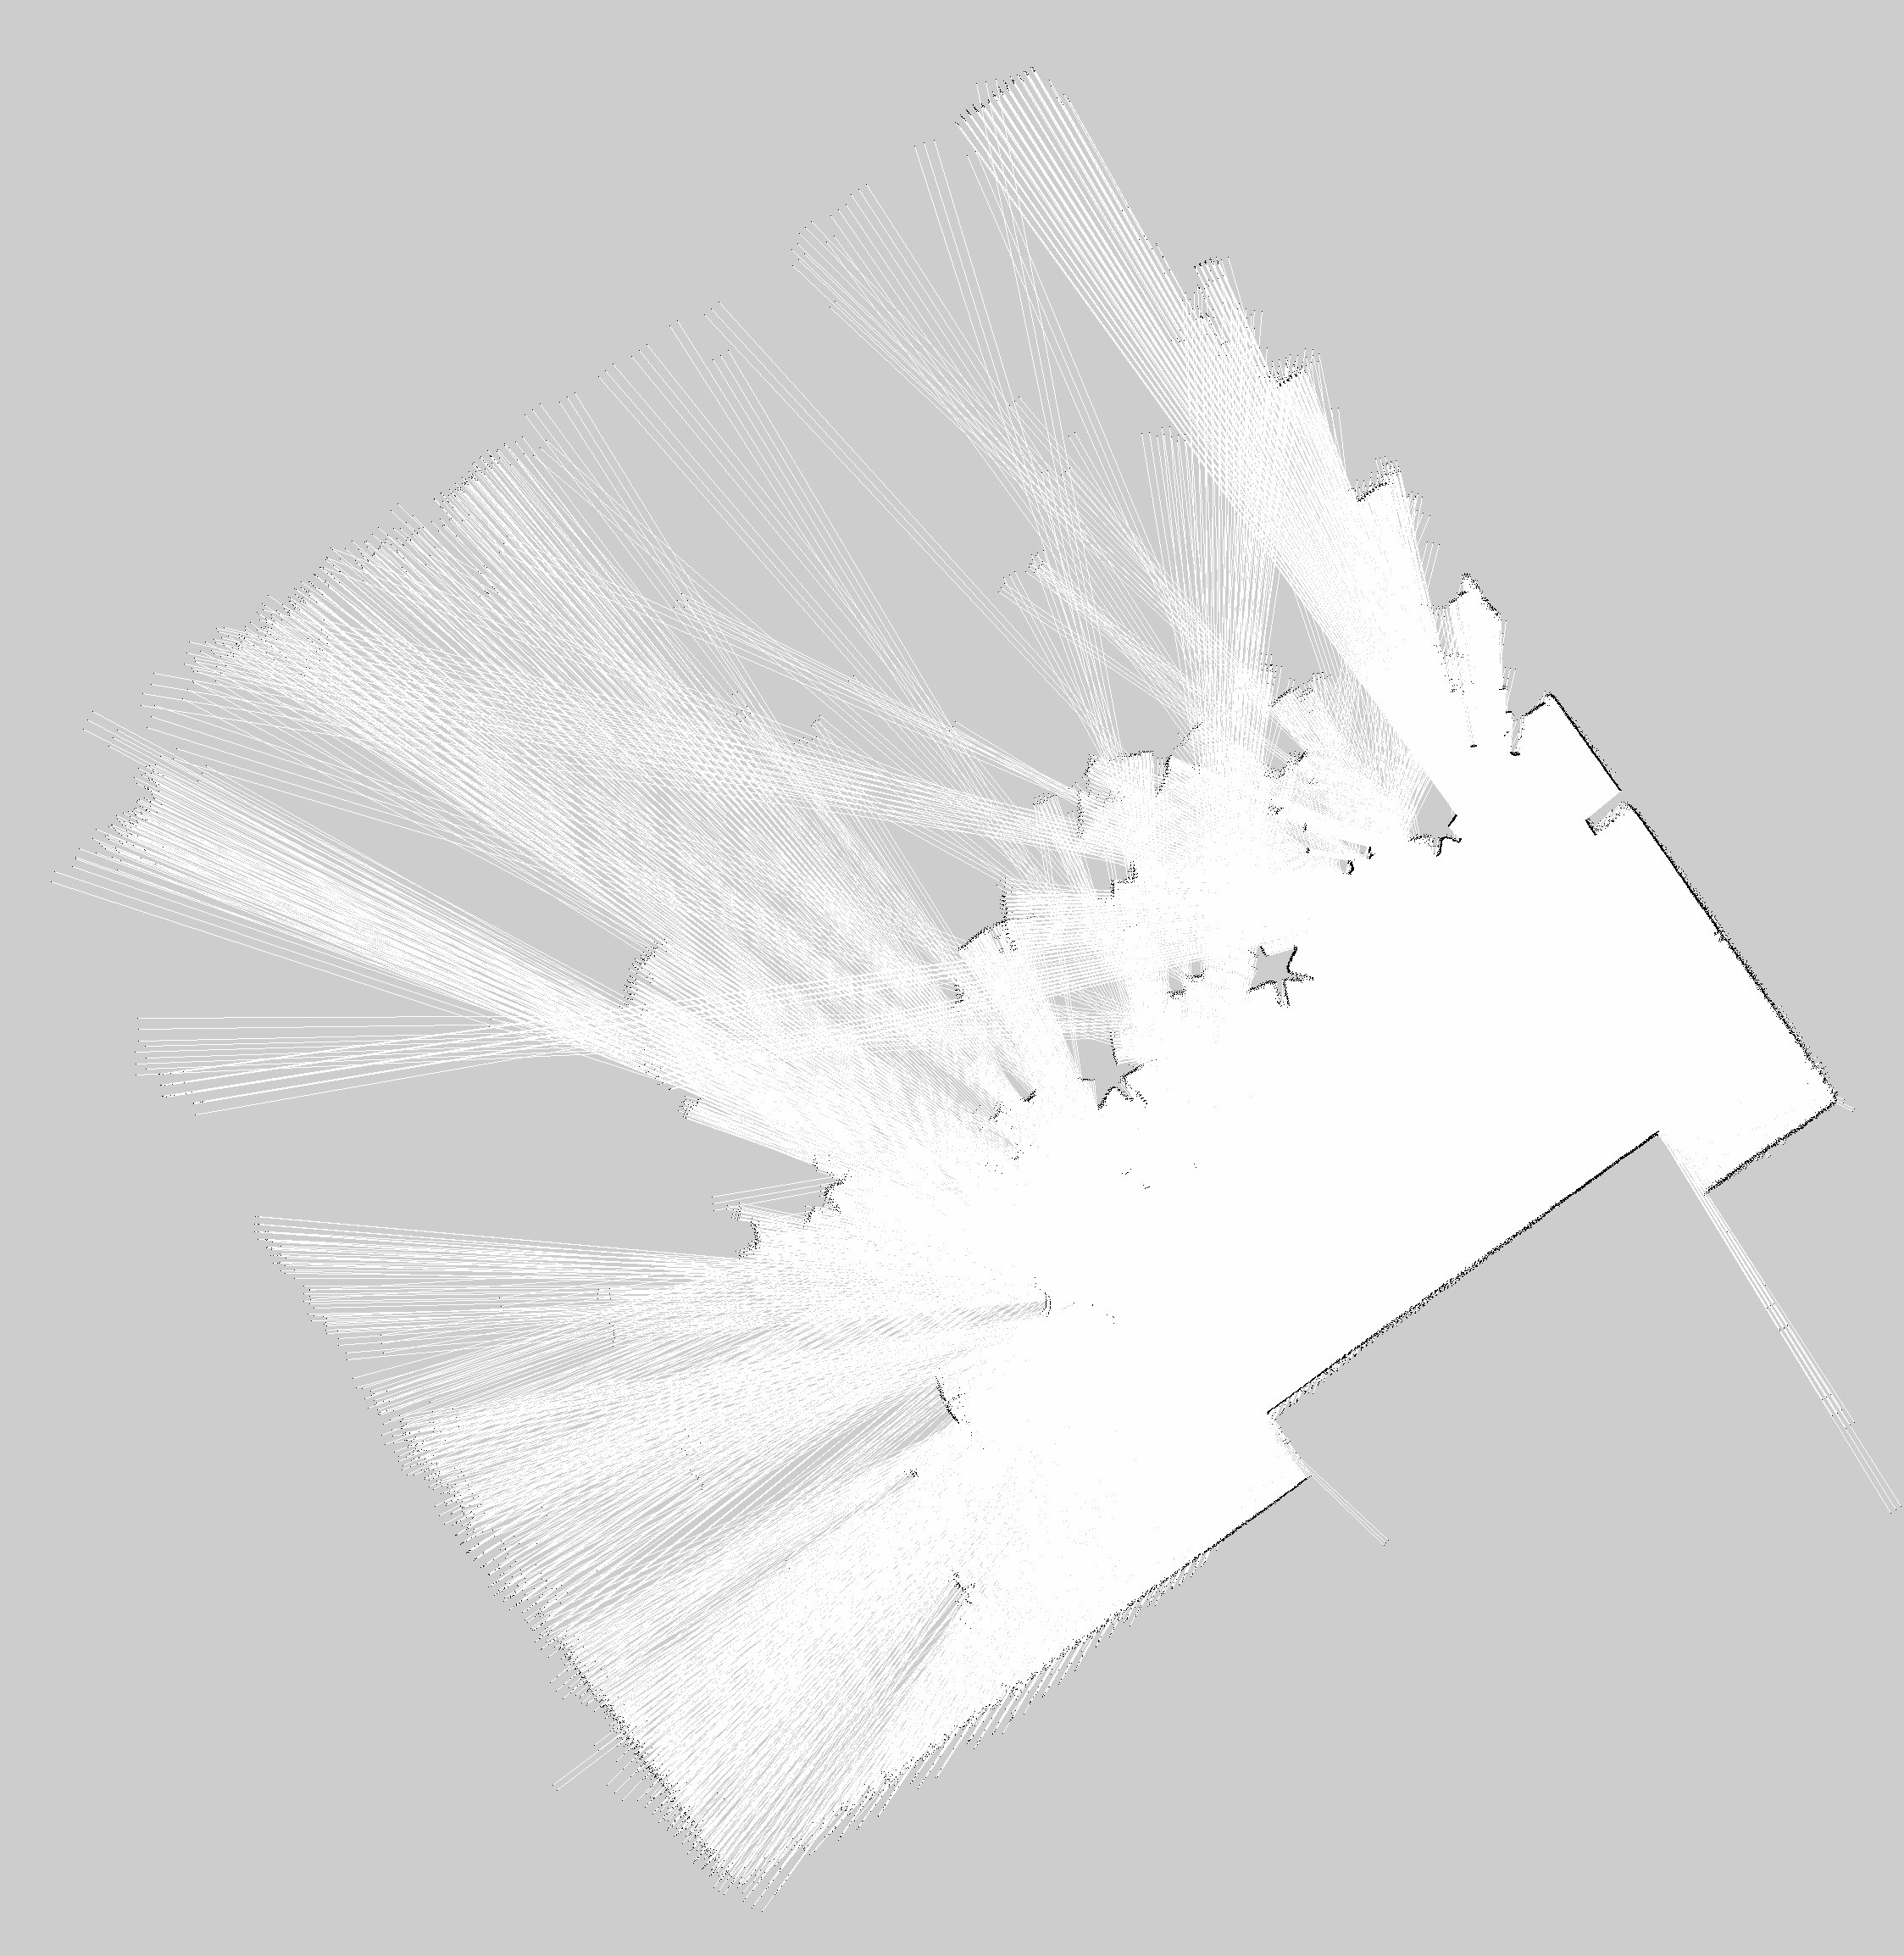
\includegraphics[width=0.8\textwidth]{Presentations/LaTeX/images/map334.jpg}
                \caption{Map of Room 334}
            \label{fig:map334}
        \end{figure}
        
    \end{minipage}  
\end{frame}

%---------------------------------------------------------------------
\section{Battery Warning}
\begin{frame}{label=bwarning}
    \frametitle{\insertsectionhead}
    \begin{itemize}
        \item Warning for battery value below 3.4V
        \item Error for battery value 3 consecutive times below 3.4V
    \end{itemize}
\end{frame}

%---------------------------------------------------------------------

\section{Setup of the navstack}
\begin{frame}[label=navstack]
	\frametitle{\insertsectionhead}%
        \begin{itemize}
        \item Followed ROS tutorial
        \item First with default planners
            \begin{itemize}
                \item Local: \ \texttt{base\_local\_planner/TrajectoryPlannerROS}
                \item Global: \texttt{navfn/NavfnROS}
            \end{itemize}
        \item New repo hamster\textunderscore2dnav
    \end{itemize}
        \begin{center}
            \begin{figure}
                    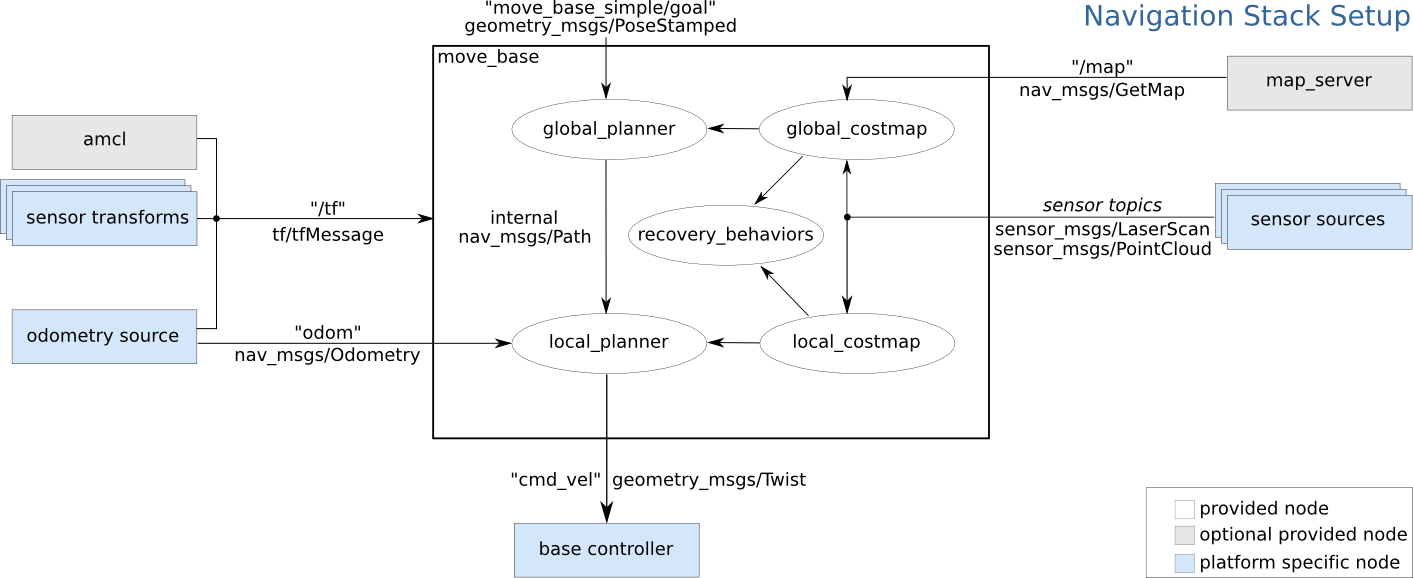
\includegraphics[width=0.6\linewidth]{Presentations/LaTeX/images/nav_stack_tutorial.png}
                    \caption{Navigation Stack on a Robot}
                    \label{fig:nav_stack_tut}
            \end{figure}
            \tiny{\url{http://wiki.ros.org/navigation/Tutorials/RobotSetup}}
        \end{center}
        

\end{frame}
%---------------------------------------------------------------------

\begin{frame}[label=challenges_navstack]
	\frametitle{\insertsectionhead}%
    \textbf{Challenges}
    \begin{itemize}
      \item<1-> \onslide<1->{  Overwriting of map:
          \begin{itemize}
            \item During trying out \texttt{move\_base.launch}
            \item Solution: run either \texttt{slam\_gmapping} or \texttt{amcl} with \texttt{move\_base}
          \end{itemize}}
      \only<2->{ \item Planner was not supporting Ackermann, 2 options:
          \begin{itemize}
            \item \texttt{sbpl\_lattice\_planner}
            \item \texttt{teb\_local\_planner}
          \end{itemize}}
      \only<3-> {\item \texttt{twist\_to\_ackermann\_node} did not work as intended
          \begin{itemize}
              \item changed file provided by cogniteam
              \item corrected conversion of velocity input into steering angle
          \end{itemize}}
    \end{itemize}
\end{frame}
%---------------------------------------------------------------------
\section{Planner integration}
\subsection{SBPL}
\begin{frame}[label=sbpl]
	\frametitle{\insertsectionhead}%
    \begin{minipage}{0.7\textwidth}
        \textbf{\insertsubsectionhead}
        \begin{itemize}
            \item No tutorial
            \begin{itemize}
                \item Installed node and tried to integrate it
            \end{itemize}
            \item SBPL requires motion primitive file
            \begin{itemize}
                \item Was not provided by Cogniteam
                \item Generation by matlab script, but just for robots turning in place
            \end{itemize}
        \end{itemize}
    \end{minipage}%
    \begin{minipage}{0.3\textwidth}
        \begin{figure}
            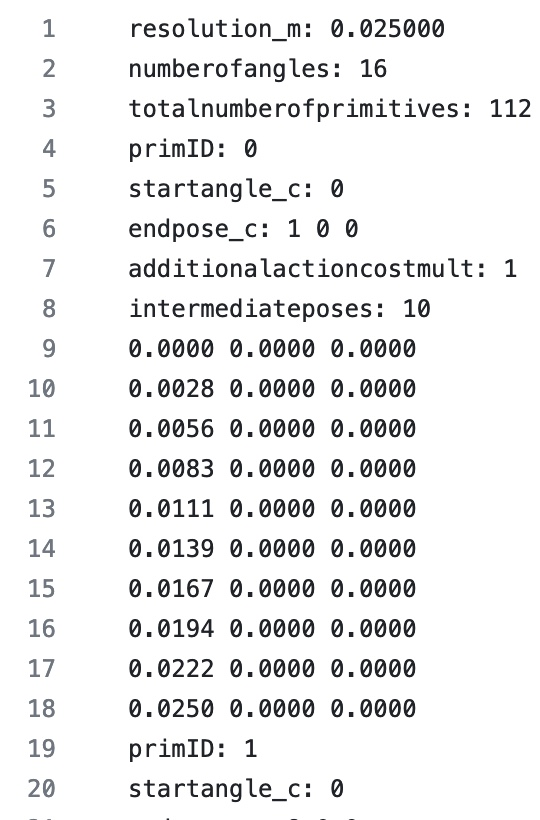
\includegraphics[width = \textwidth]{Presentations/LaTeX/images/mprim.jpeg}
            \caption{mprim file}
        \end{figure}
    \end{minipage}
\end{frame}
%---------------------------------------------------------------------
\subsection{TEB}
\begin{frame}[label=teb]
	\frametitle{\insertsectionhead}%
     \begin{minipage}{0.7\textwidth}
        \textbf{\insertsubsectionhead}
        \begin{itemize}
          \item Timed Elastic Band method
          \item Non-holonomic and kinematic constraints of vehicles
          \item Obstacle avoidance using costmaps
          \item Variety of customizable parameters
          \item Compatible with ROS \texttt{move\_base} node
        \end{itemize}
    \end{minipage}%
    \begin{minipage}{0.3\textwidth}
        \vspace{1cm}
        \begin{center}
            \begin{figure}
                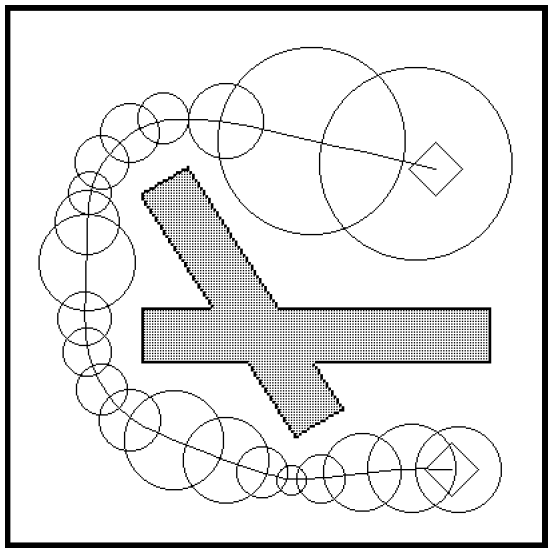
\includegraphics[width=1\linewidth]{Presentations/LaTeX/images/teb.png}
                \caption{TEB planner}
                \label{fig:teb}
            \end{figure}
            \tiny{\url{https://hackmd.io/@Unmesh/rkUi8MJMI}}
        \end{center}
    \end{minipage}
\end{frame}
%---------------------------------------------------------------------
\subsection{Challenge: localization}
\begin{frame}[label=challenge_localization]
	\frametitle{\insertsectionhead}%
         \textbf{\insertsubsectionhead}
     \begin{itemize}
        \item Inaccurate odometry provided by Cogniteam
        \begin{itemize}
            \item Due to Ackermann-steering the localization by odometry did not work
            \item Localization should work just with LaserScan
        \end{itemize}
        \item \texttt{laser\_scan\_matcher}
        \begin{itemize}
            \item Create fake odometry to be provided to amcl for localization
        \end{itemize}
     \end{itemize}
\end{frame}

% ---------------------------------------------------------------------
\begin{frame}[label=video]
	\frametitle{\insertsectionhead}
         \textbf{\insertsubsectionhead}
    \begin{center}
          \includemedia[
      width=0.7\linewidth,
      height=0.4549\linewidth,
      activate=pageopen,
      addresource=Presentations/LaTeX/images/video.mp4,
      flashvars={source=Presentations/LaTeX/images/video.mp4}
    ]{}{VPlayer.swf}  
    \end{center}
\end{frame}

%---------------------------------------------------------------------
\subsection{TEB parametrization}
\begin{frame}{label=teb_param}
    \frametitle{\insertsectionhead}
    \textbf{\insertsubsectionhead}
    \begin{itemize}
        \item Minimum turning radius
        \item Publish feedback (for rviz)
        \item Maximum acceleration
        \item Wheelbase
        \item Goal tolerance (angle and euclidean distance)
        \item Min\_obstacle\_dist
    \end{itemize}
\end{frame}

%---------------------------------------------------------------------
\section{Emergency Stop}
\begin{frame}{label=estop}
    \frametitle{\insertsectionhead}
    \begin{minipage}{0.4\textwidth}
        \begin{itemize}
            \item<1-> Robot stops when there are points registered:
            \begin{itemize}
                \item Between min\_angle and max\_angle
                \item Nearer than obstacle\_distance
            \end{itemize}
            \only<3->{\item \texttt{twist\_mux} to get correct priorities for input}
        \end{itemize}
    \end{minipage}%
    \begin{minipage}{0.6\textwidth}
    \begin{center}
        \vspace{0.5cm}
        \begin{figure}
            \begin{overprint}
                \onslide<1>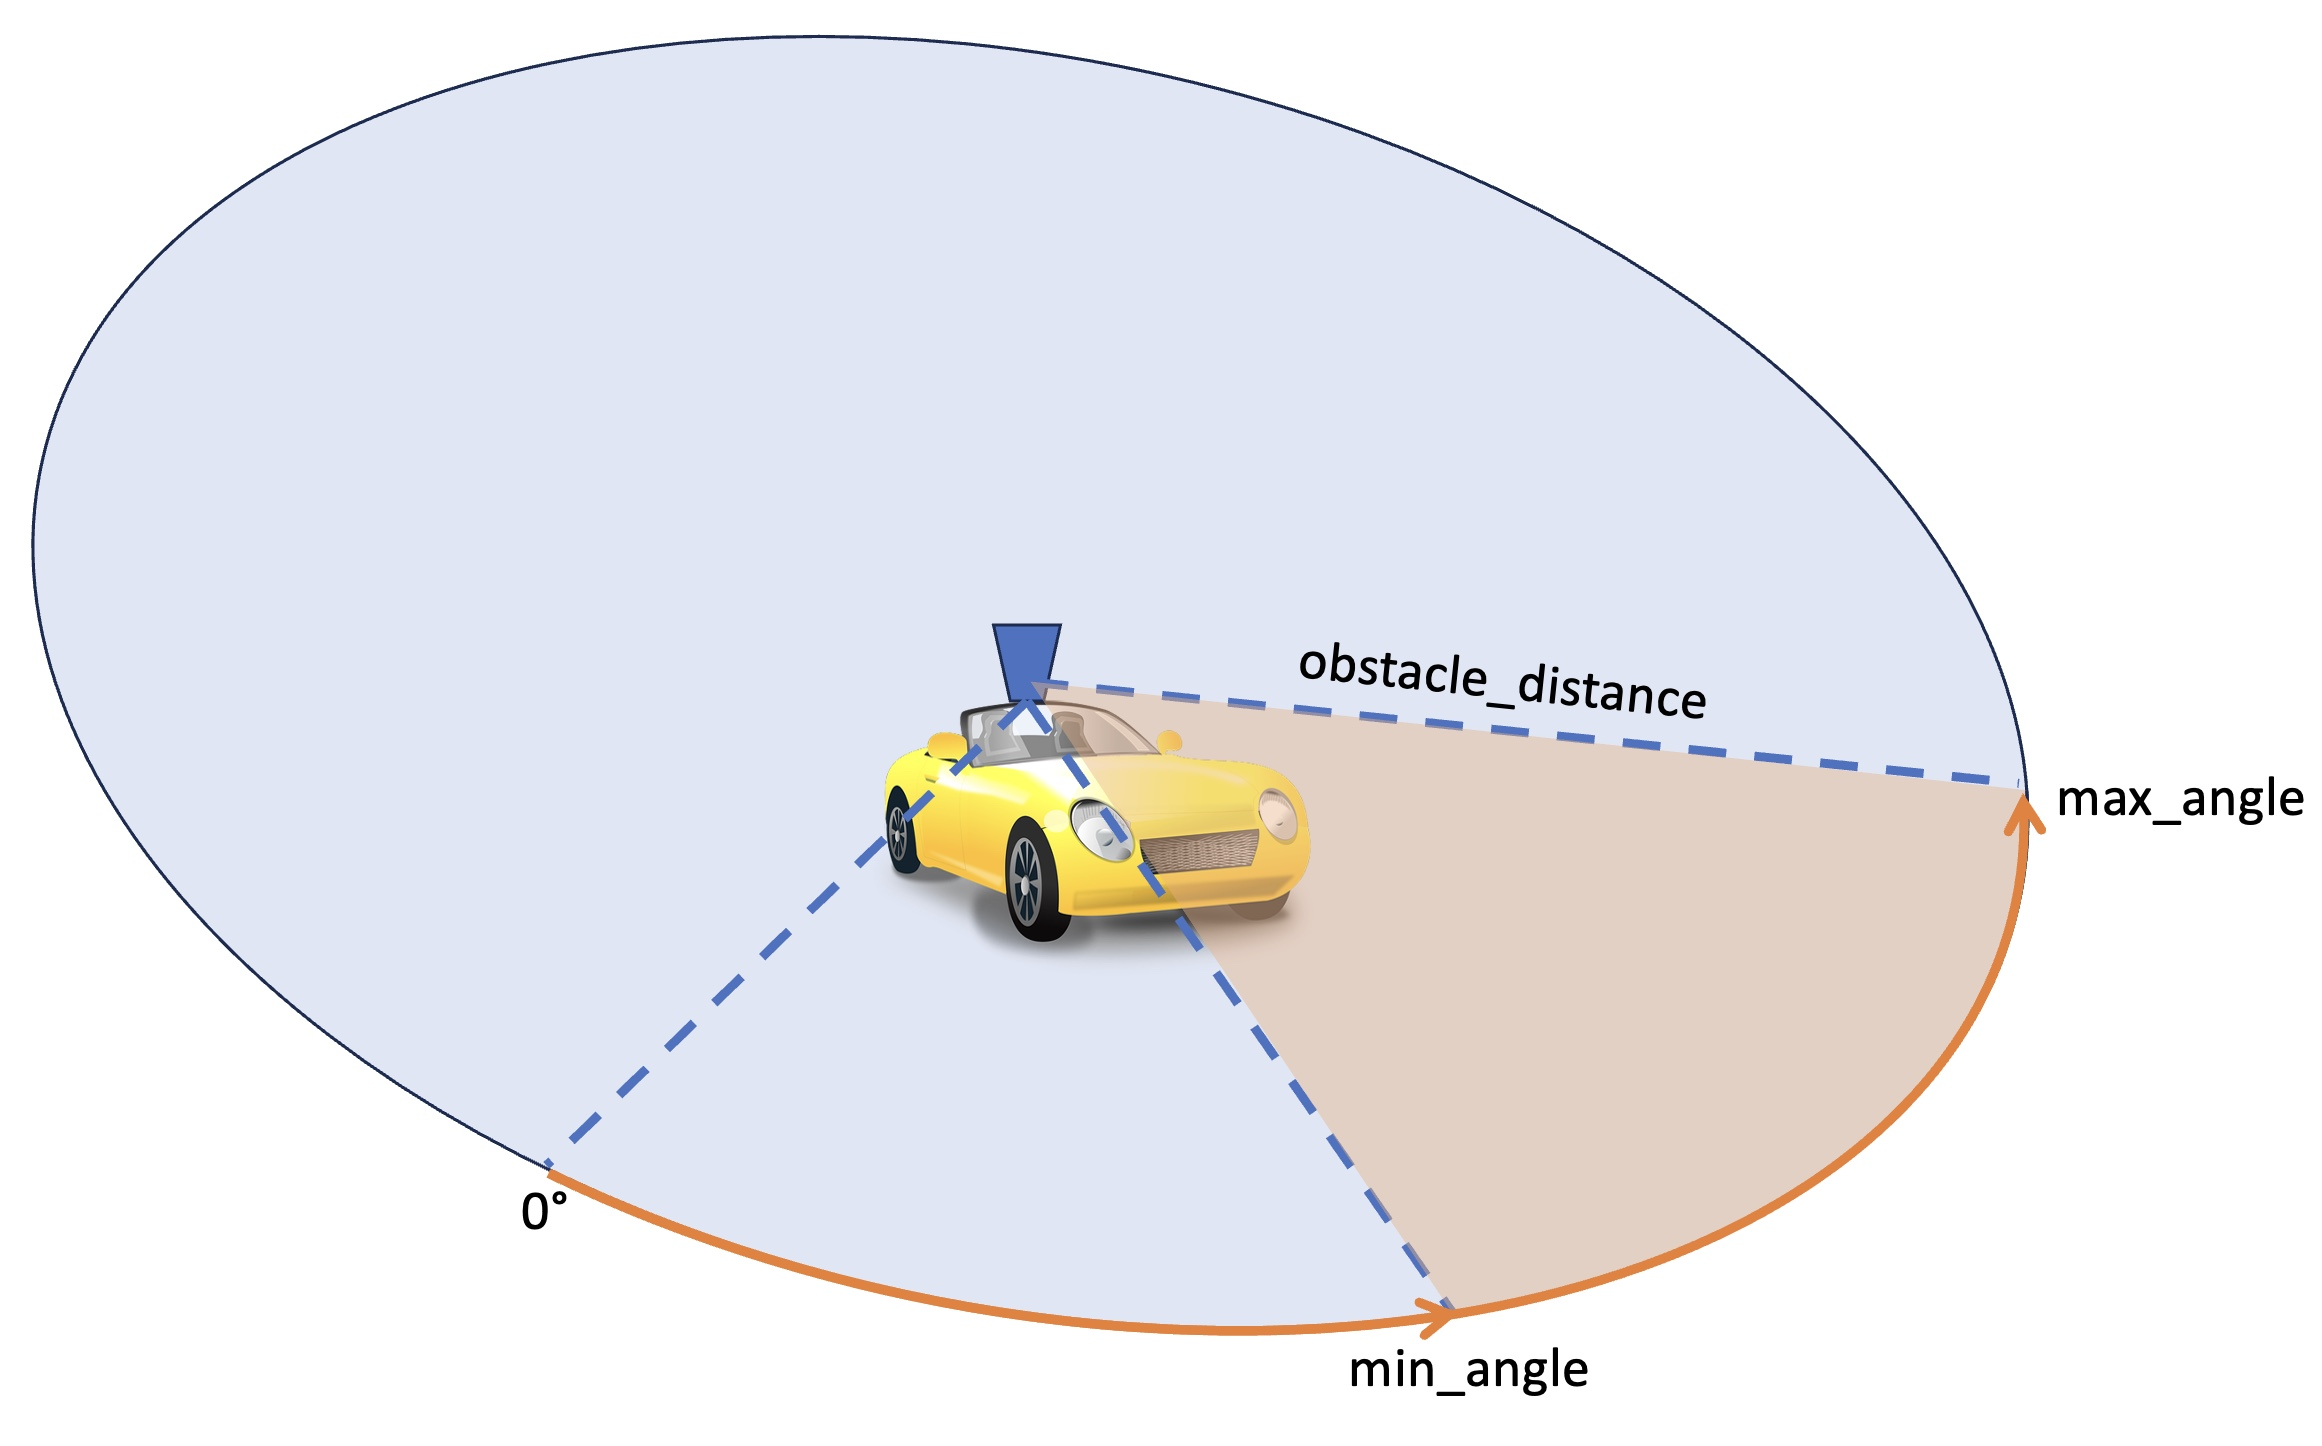
\includegraphics[width=\textwidth]{Presentations/LaTeX/images/estop-normal.jpeg}
                    \caption{Anglular parameters}
                \onslide<2>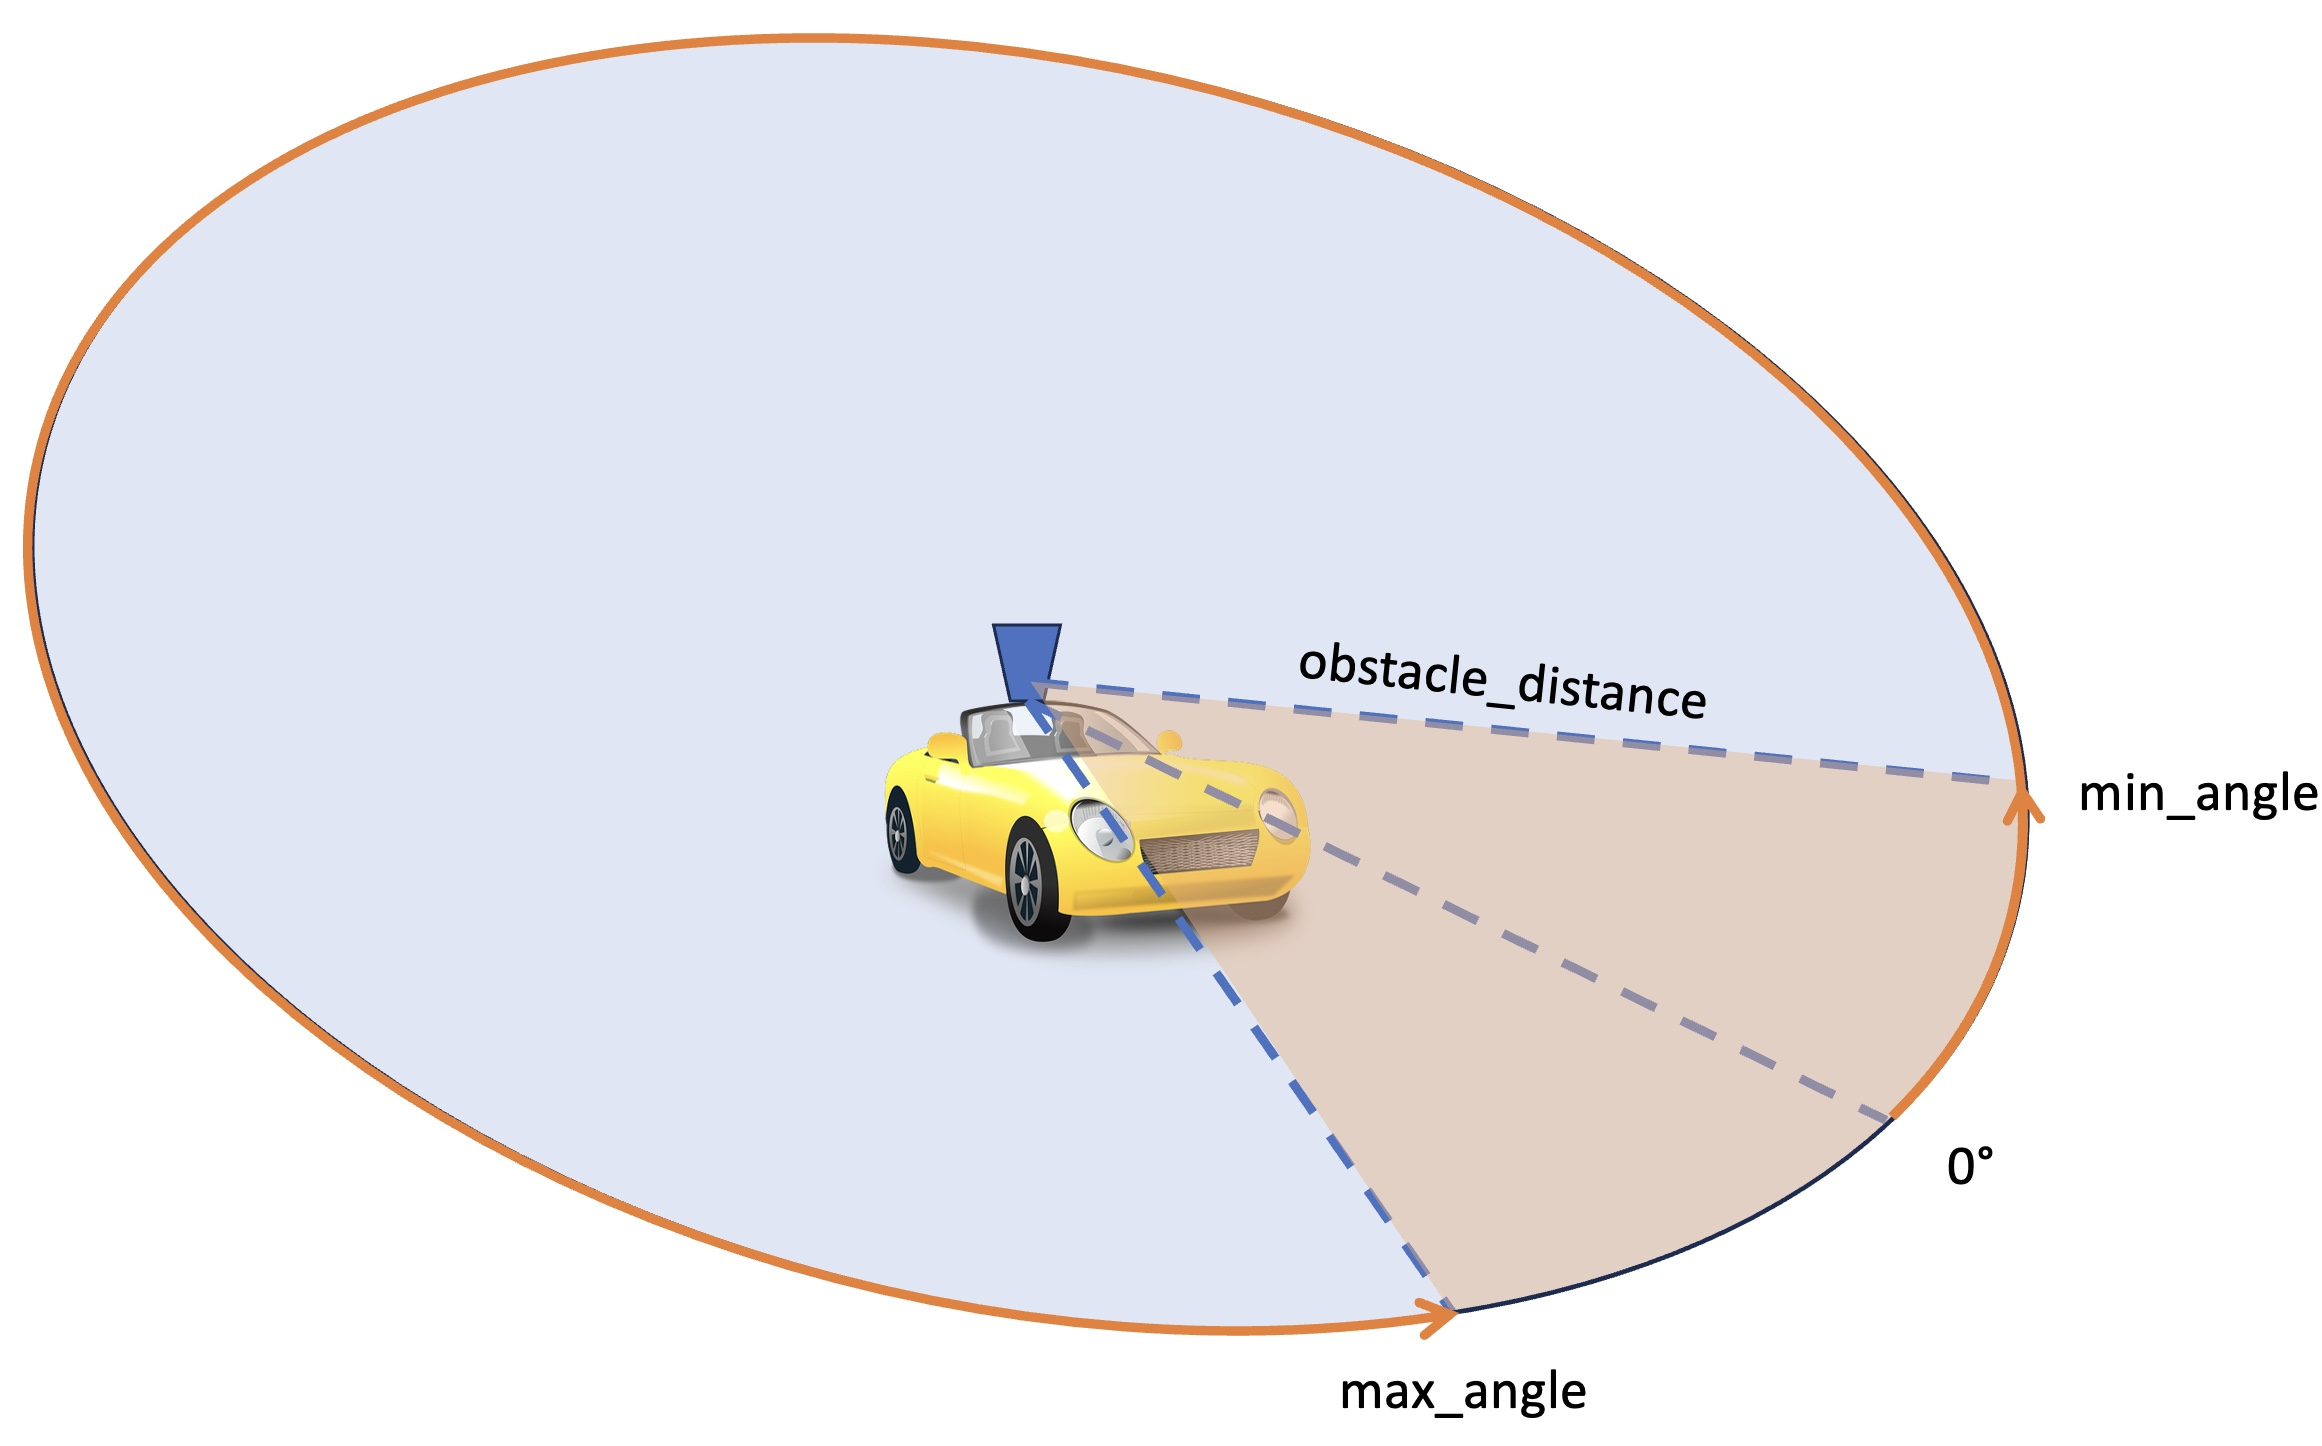
\includegraphics[width=\textwidth]{Presentations/LaTeX/images/estop-ausnahmefall.jpeg}
                    \caption{Angular parameters: special case}
                \onslide<3>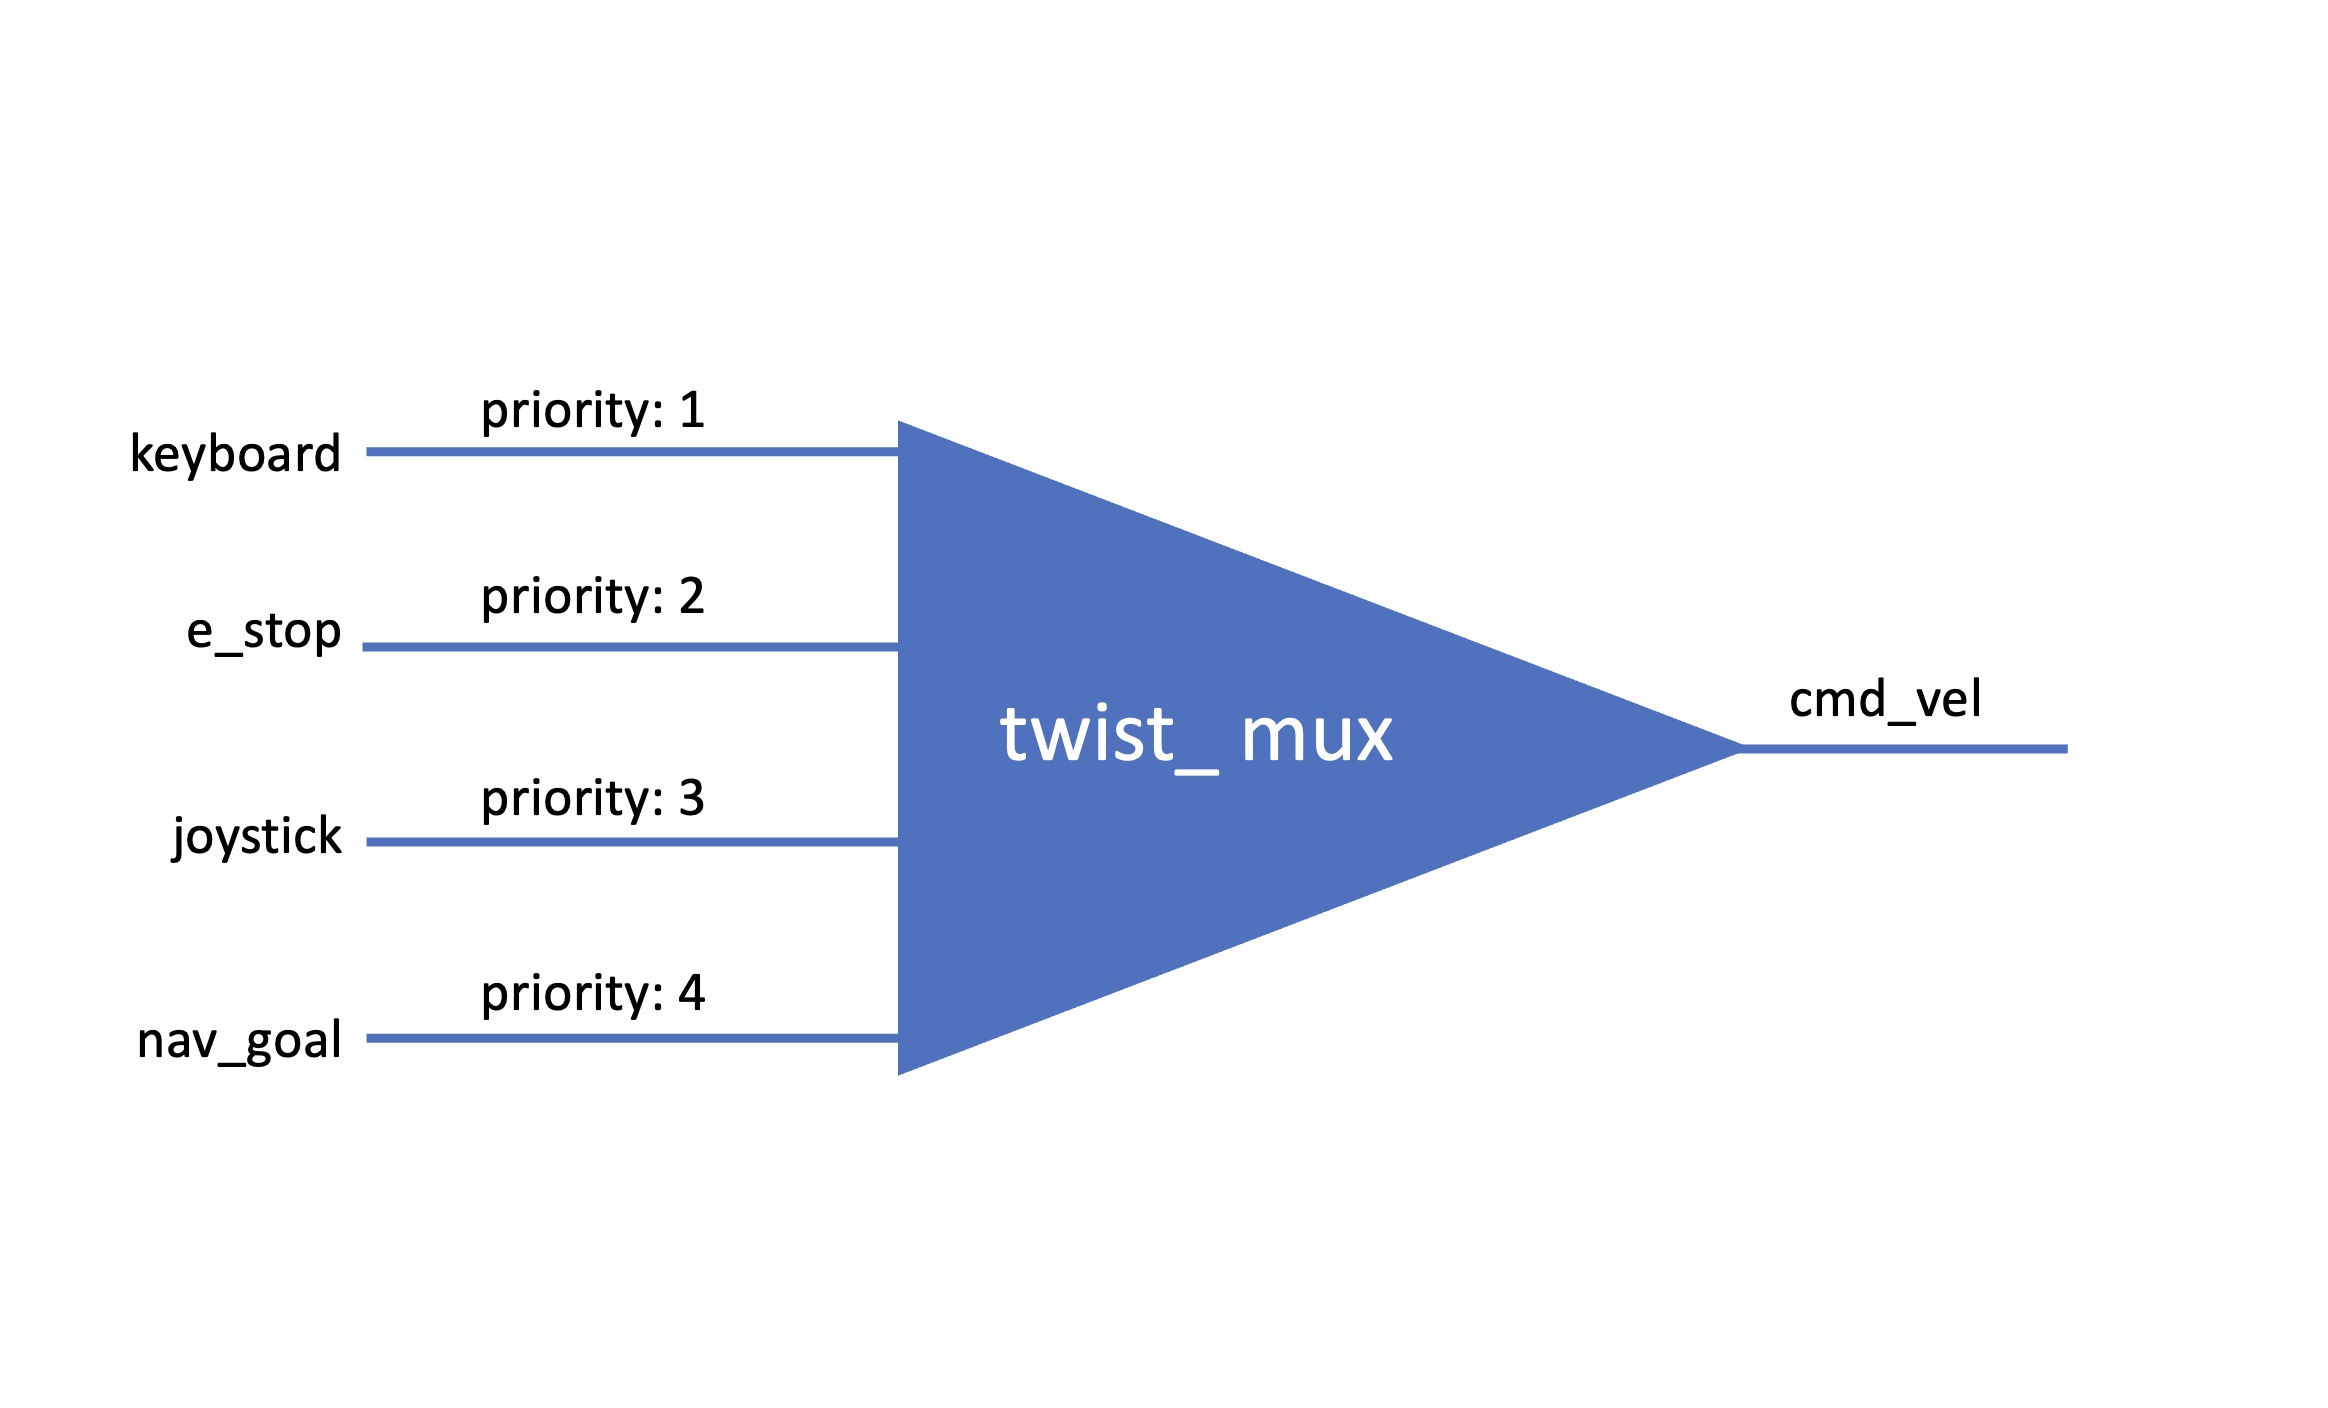
\includegraphics[width=\textwidth]{Presentations/LaTeX/images/twist_mux.jpeg}
                    \caption{Structure of the twist\_mux}
                    \label{fig:tmux}
            \end{overprint}
            
        \end{figure}
    \end{center}
    \end{minipage}
\end{frame}

% %---------------------------------------------------------------------
% \begin{frame}{label=estop_1}
%     \frametitle{\insertsectionhead}
%     \begin{center}
%         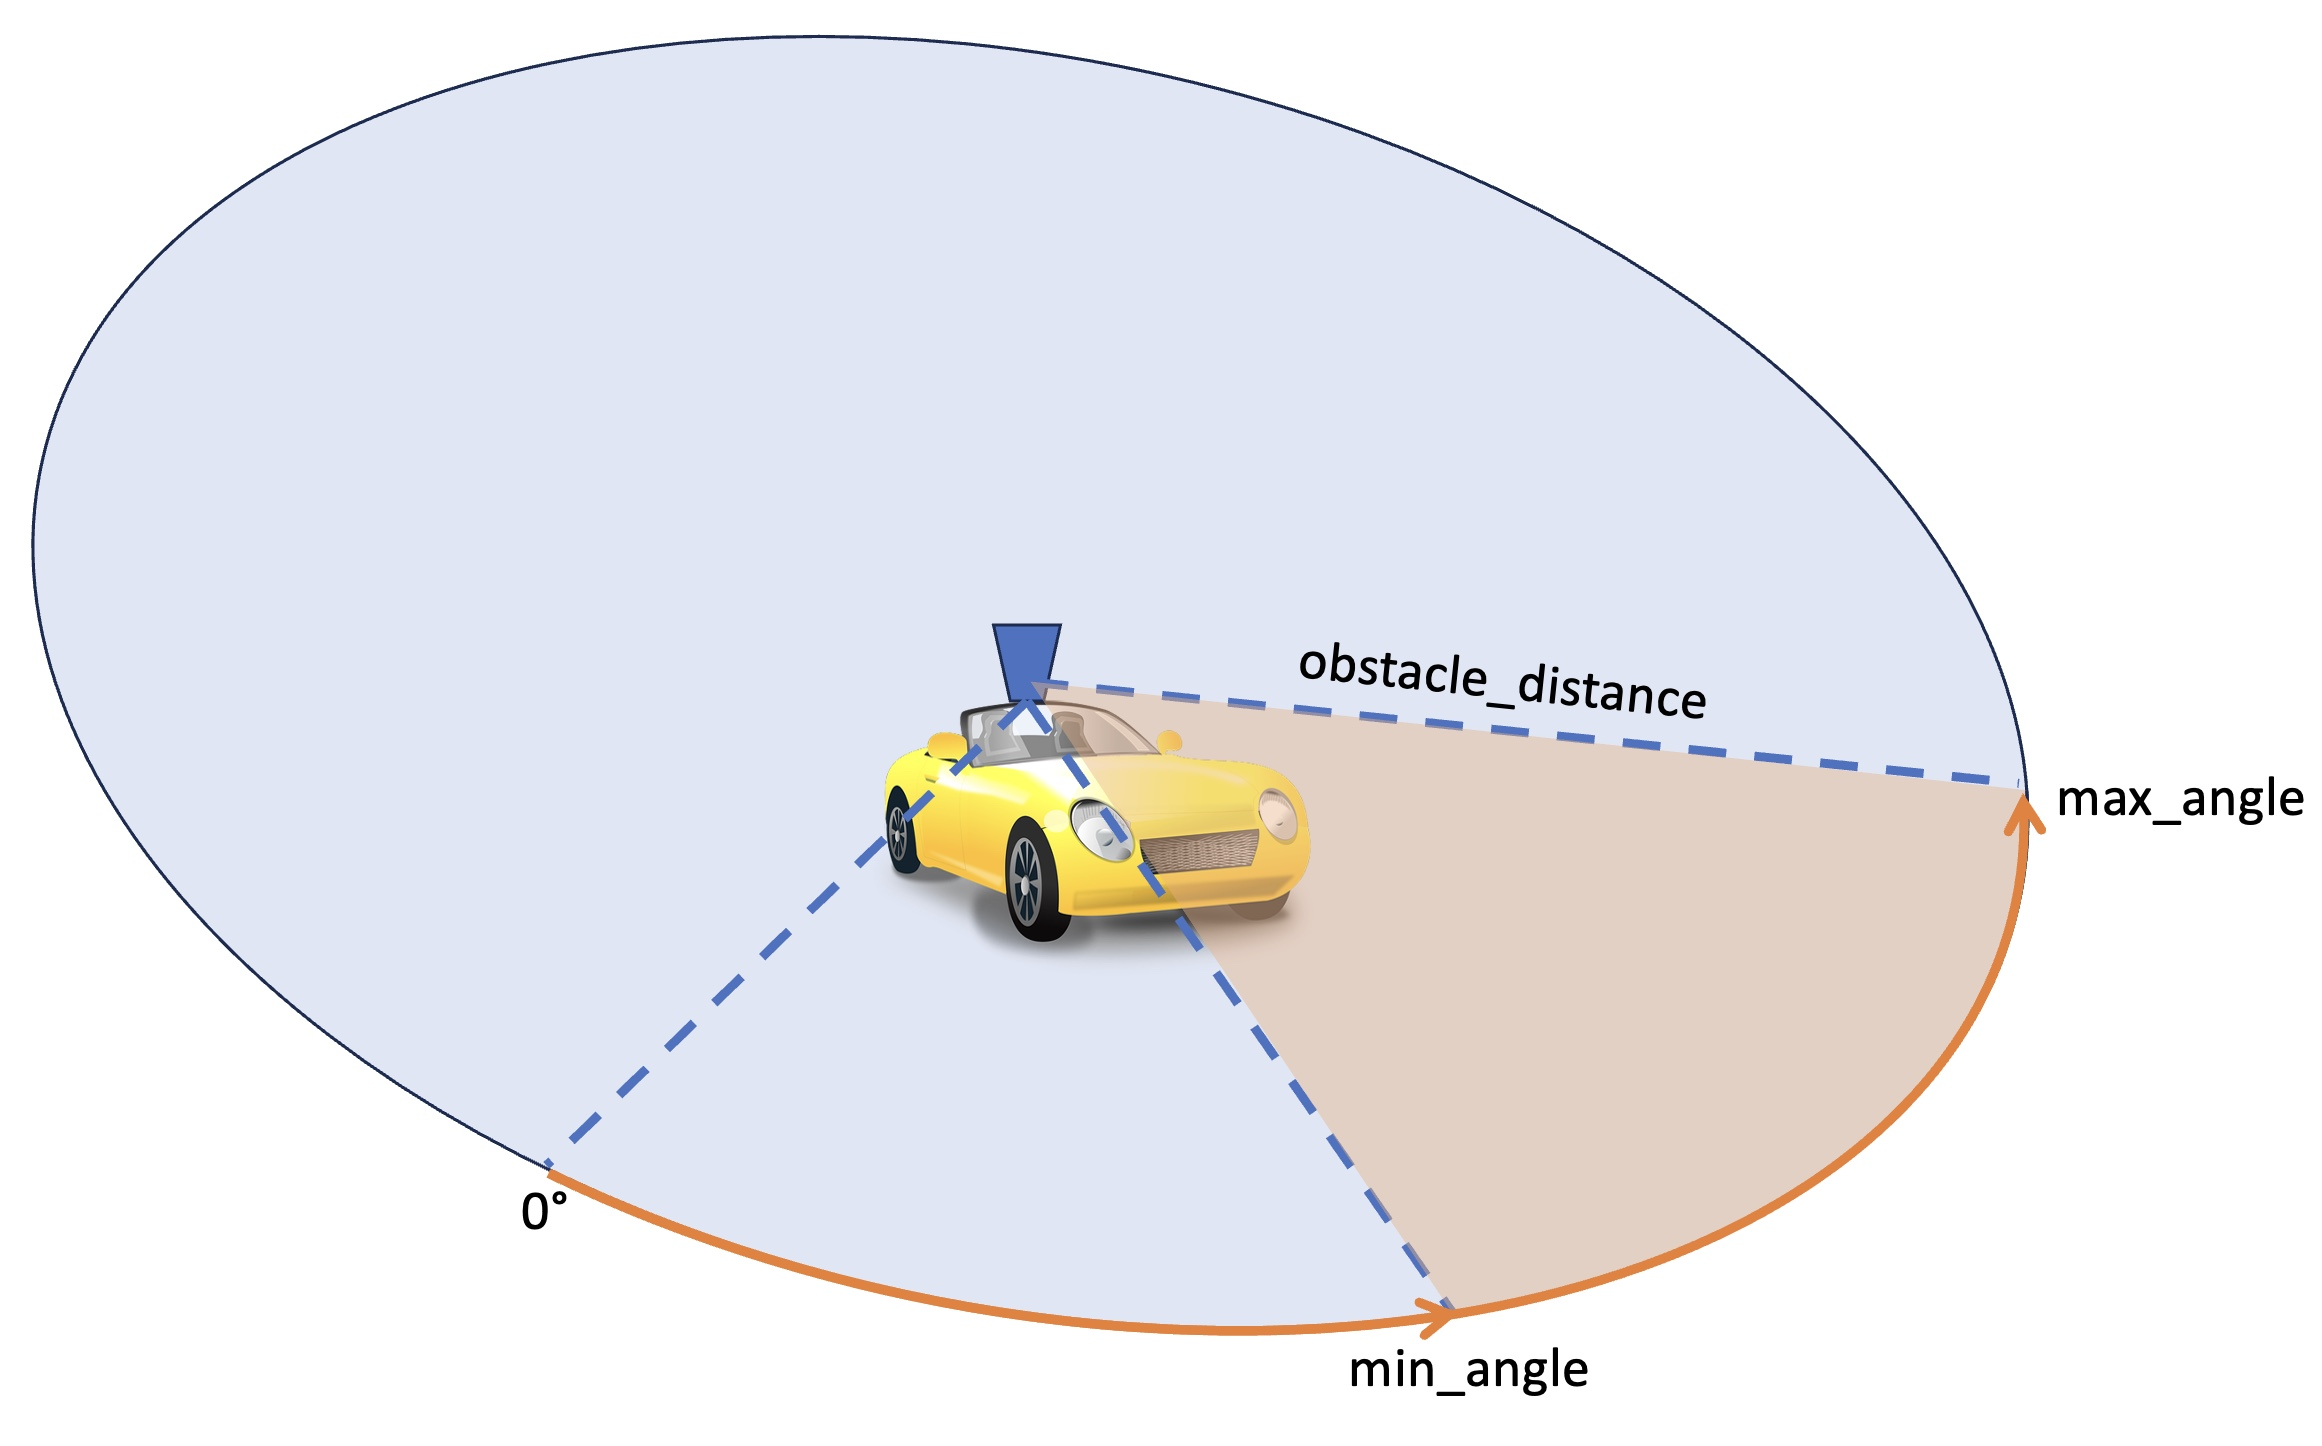
\includegraphics[width=0.8\textwidth]{Presentations/LaTeX/images/estop-normal.jpeg}
%     \end{center}
% \end{frame}

% %---------------------------------------------------------------------
% \begin{frame}{label=estop_2}
%     \frametitle{\insertsectionhead}
%     \begin{center}
%         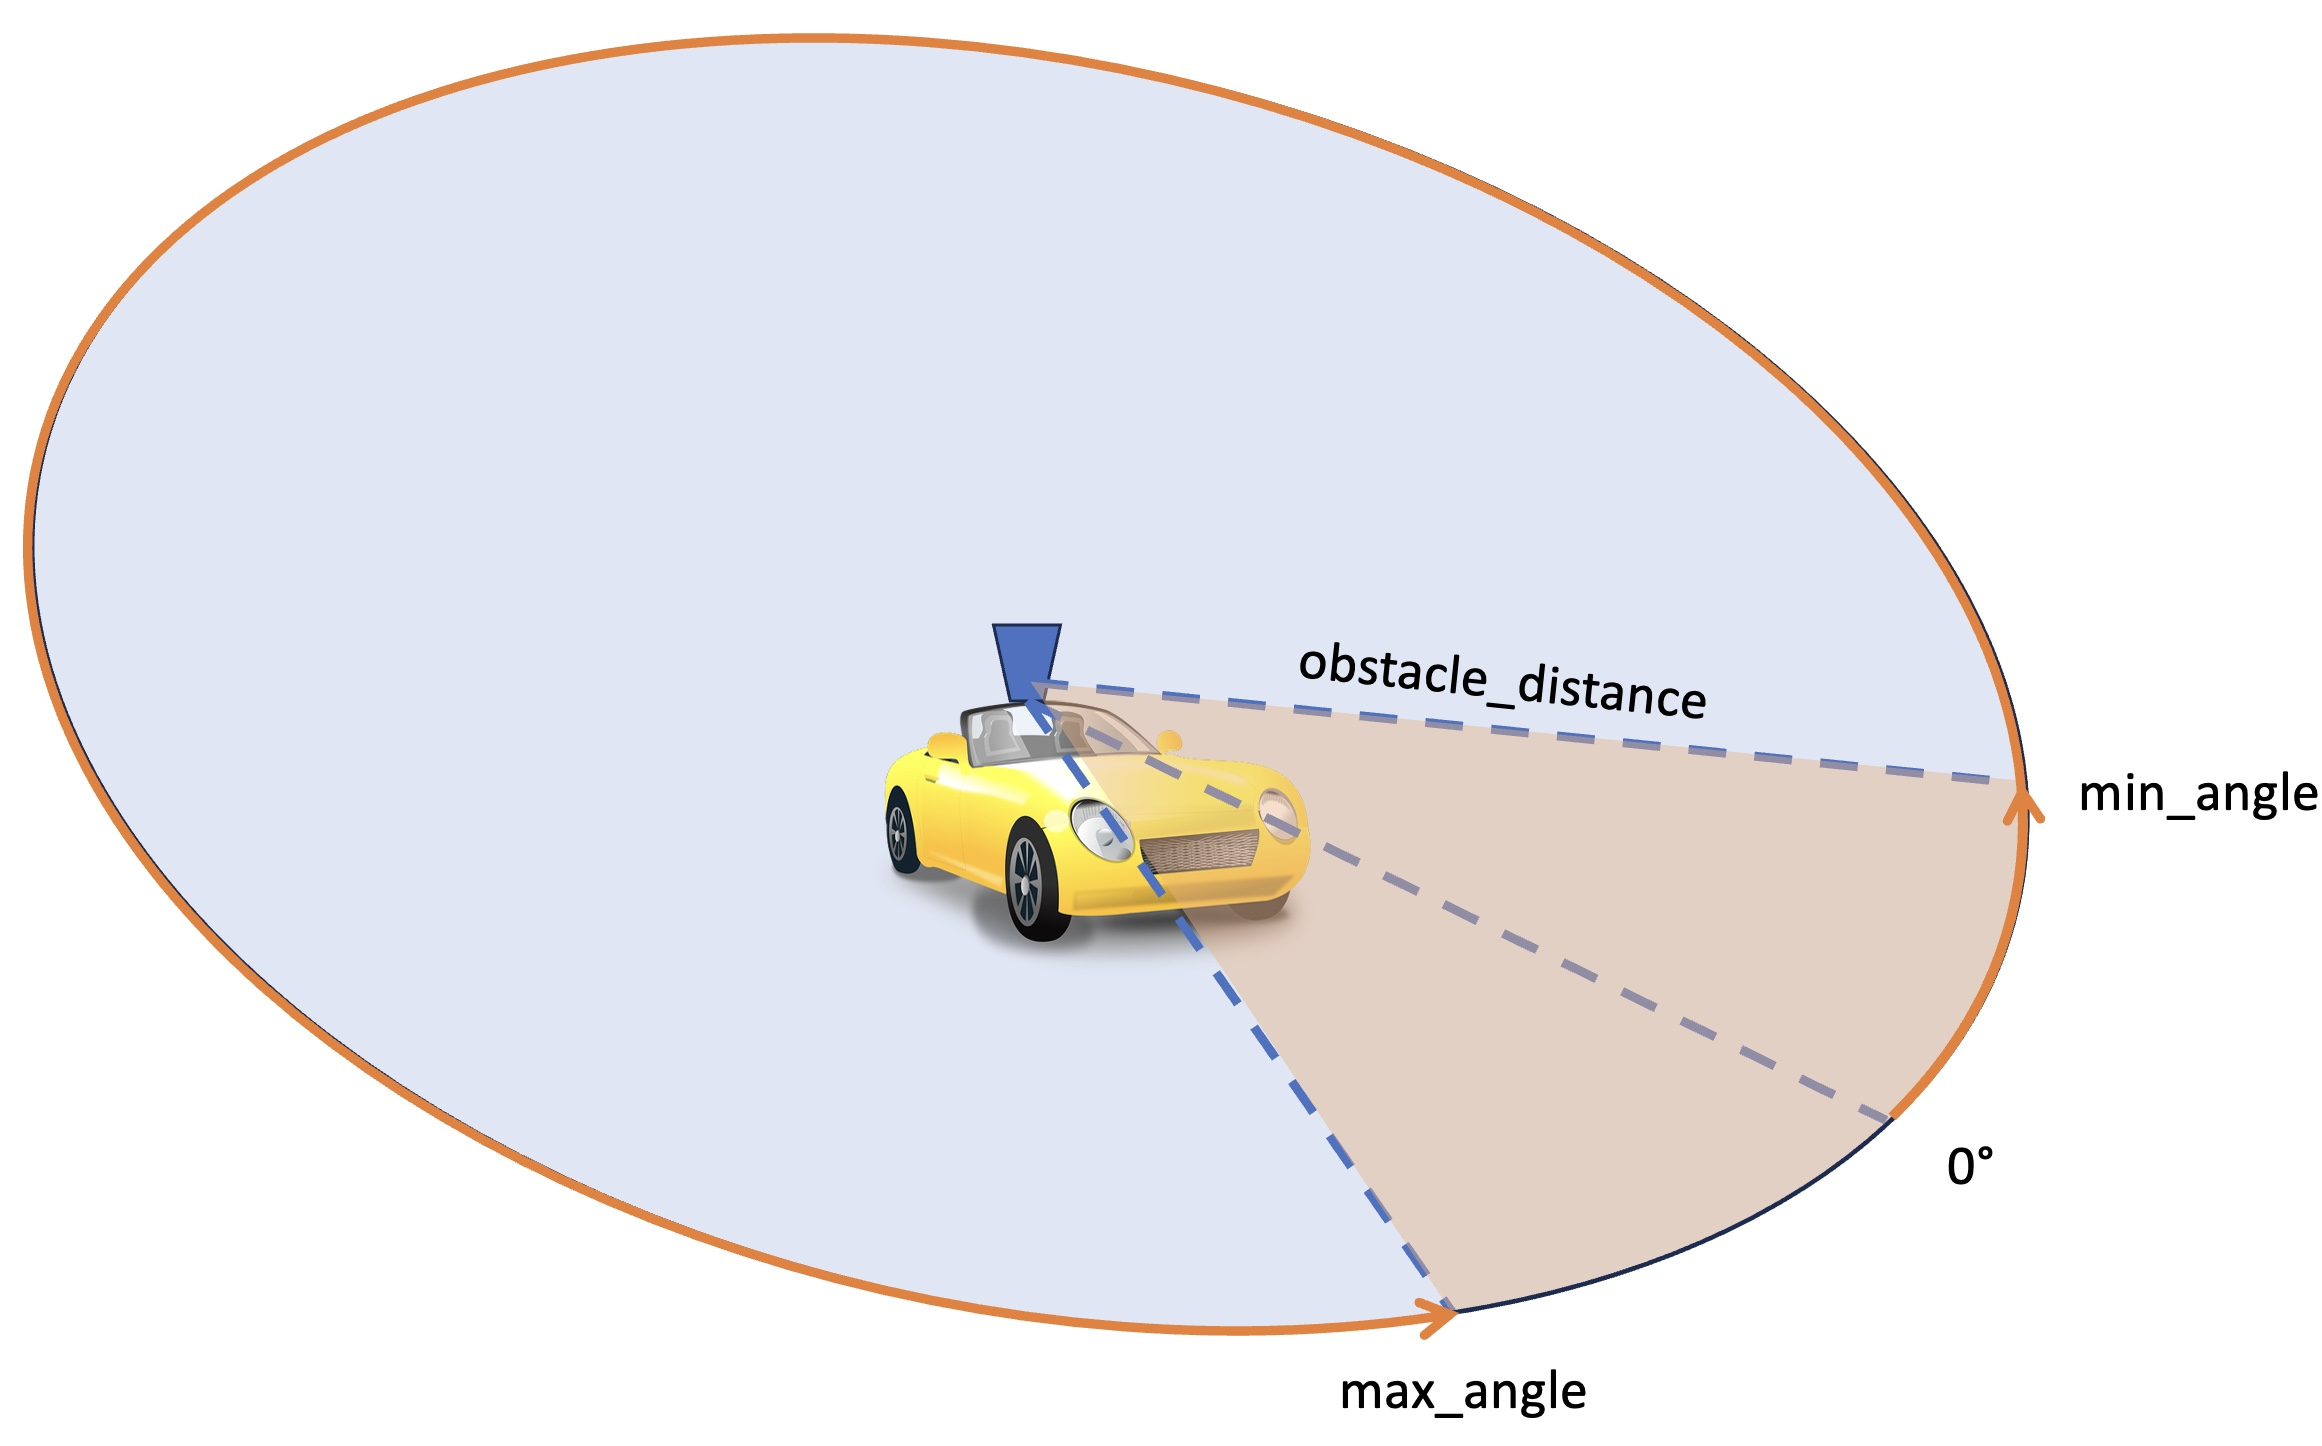
\includegraphics[width=0.8\textwidth]{Presentations/LaTeX/images/estop-ausnahmefall.jpeg}
%     \end{center}
% \end{frame}

%---------------------------------------------------------------------
% \subsection{Point Cloud}
% \begin{frame}{label=point_cloud}
%     \frametitle{\insertsectionhead}
%     \textbf{\insertsubsectionhead}
%     \begin{itemize}
%         \item Camera doesn’t acquire point cloud data but depth images
%         \item Hardware does not allow working with point clouds
%         \item If hardware allows using point clouds: package laserscan-to-pointcloud
%         \item Implement nodes that subscribe to data input and publish LaserScan data to next node (emergency stop)

%     \end{itemize}
% \end{frame}

%%%%%%%%%%%%%%%%%%%%%%%%%%%%%%%%%%%%%%%%%%%%%%%%%%%%%%%%%%%%%%%%%%%%%%%%%
%
% Thank you slide
%
%%%%%%%%%%%%%%%%%%%%%%%%%%%%%%%%%%%%%%%%%%%%%%%%%%%%%%%%%%%%%%%%%%%%%%%%%

\begingroup% to remove header and footline and include style of first slide
\setbeamertemplate{header}{}
\setbeamertemplate{footline}{}
\begin{frame}[label=overview]
	\frametitle{Thank You For Your Attention!}%
	\begin{tikzpicture}[overlay, remember picture, shift={(current page.south west)}, inner sep=0pt, outer sep=0pt]

		\useasboundingbox (0,0) rectangle (160mm,90mm);%

		\node[anchor=south east] at (150mm,7mm) {\includegraphics[width=50mm]{logos/AMS.pdf}};%

		\fill[ovgu-inf-blue] (0,90mm) rectangle (160mm,55mm);
		\node[anchor=north east] at (160mm,90mm) {\includegraphics{./logos/otto.pdf}};
		% \makeatletter
		\node[anchor=north west] at (14mm,87mm) {\includegraphics[height=11mm]{./logos/Signet_INF_1_inv.pdf}};	
		% \makeatother
		\node[anchor=south west, text width=160mm-28mm] at (14mm,55mm+5mm) {\color{white}\usebeamerfont{title}\inserttitle\par};

		\node[anchor=north west, text width=160mm-28] at (14mm,55mm-15mm) {%
			{\usebeamerfont{title}\color{AMSblue}\insertframetitle\par}%
		};			

	

	\end{tikzpicture}
    % \Notes{

    % }
    \transfade[duration=5]%<2->
\end{frame}	
\endgroup

\end{document}
